\documentclass[12pt]{article}
\usepackage{amsmath,amsfonts}
\usepackage{enumerate}
\usepackage{graphicx}

\renewcommand{\baselinestretch}{1}
\topmargin 0in \headheight 0.0in \textheight 9in \textwidth 6.5in
\oddsidemargin 0.1in \evensidemargin 0.1in

\begin{document}

\section*{Data Generation}

The dataset contains 2000 simulated images, with 1000 images each in groups A and B. Each image has 256 pixels arranged in a \(16 \times 16\) grid. The \(\beta\) matrix, set to 1 in an \(8 \times 8\) central region and 0 elsewhere, modifies the pixel values in group A. The \texttt{group\_ind} vector differentiates the groups, assigning 1 to group A and 0 to group B. Noise \(\epsilon_i\), generated from a multivariate normal distribution with zero mean and a covariance matrix from an exponential correlation function with rate 1, is added to the pixel values.

To adapt the data for the input specifications of the \texttt{myresf\_vc} function, the dataset was transformed into a long format. In this format, the columns \texttt{x} and \texttt{y} denote the coordinates, while \texttt{pixel\_value} corresponds to the simulated $y$ values.

\section*{VBM}

In the VBM analysis, a Generalized Linear Model (GLM) was applied pixel-wise to assess group effects on pixel intensities across 100 iterations. For each iteration, the model generated effect size estimates and p-values for each pixel. These p-values were then corrected for multiple comparisons using the Bonferroni method. Figure \ref{fig:vbm_pvals} depicts the frequency of significant p-values in across pixels, with pixels showing significant \(\beta\) in all 100 iterations appearing in black, and those never showing significance in white.

\begin{figure}[ht]
    \centering
    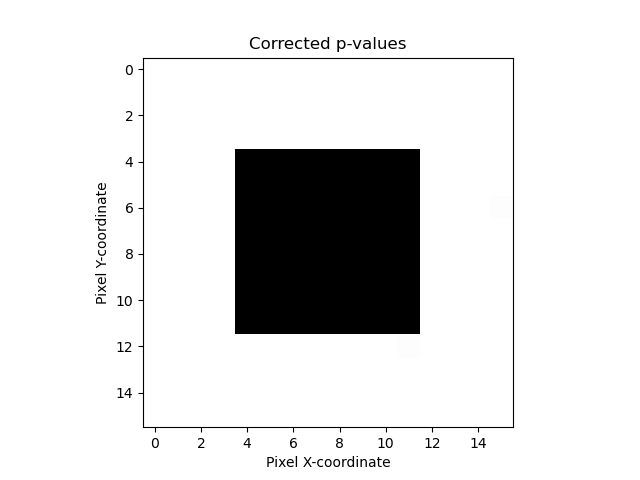
\includegraphics[width=0.5\textwidth]{/Users/siyangren/Documents/ra-cida/ESFGSP_Paper/Figures/vbm_pvals.png}
    \caption{}
    \label{fig:vbm_pvals}
\end{figure}

\begin{figure}[ht]
    \centering
    % First figure
    \begin{minipage}[b]{0.45\textwidth}
        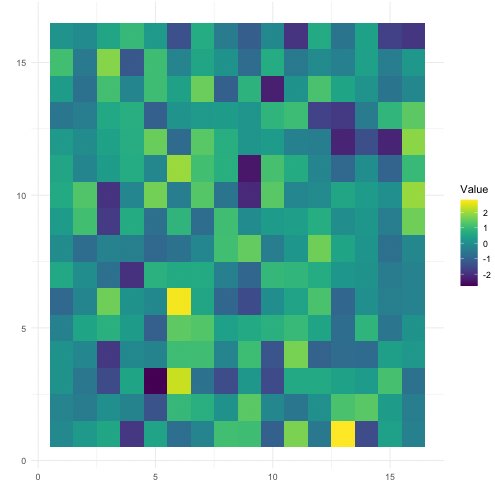
\includegraphics[width=\textwidth]{/Users/siyangren/Documents/ra-cida/ESFGSP_Paper/Figures/image_ex1.png}
    \end{minipage}
    \hfill % This command adds a space between the two figures
    % Second figure
    \begin{minipage}[b]{0.45\textwidth}
        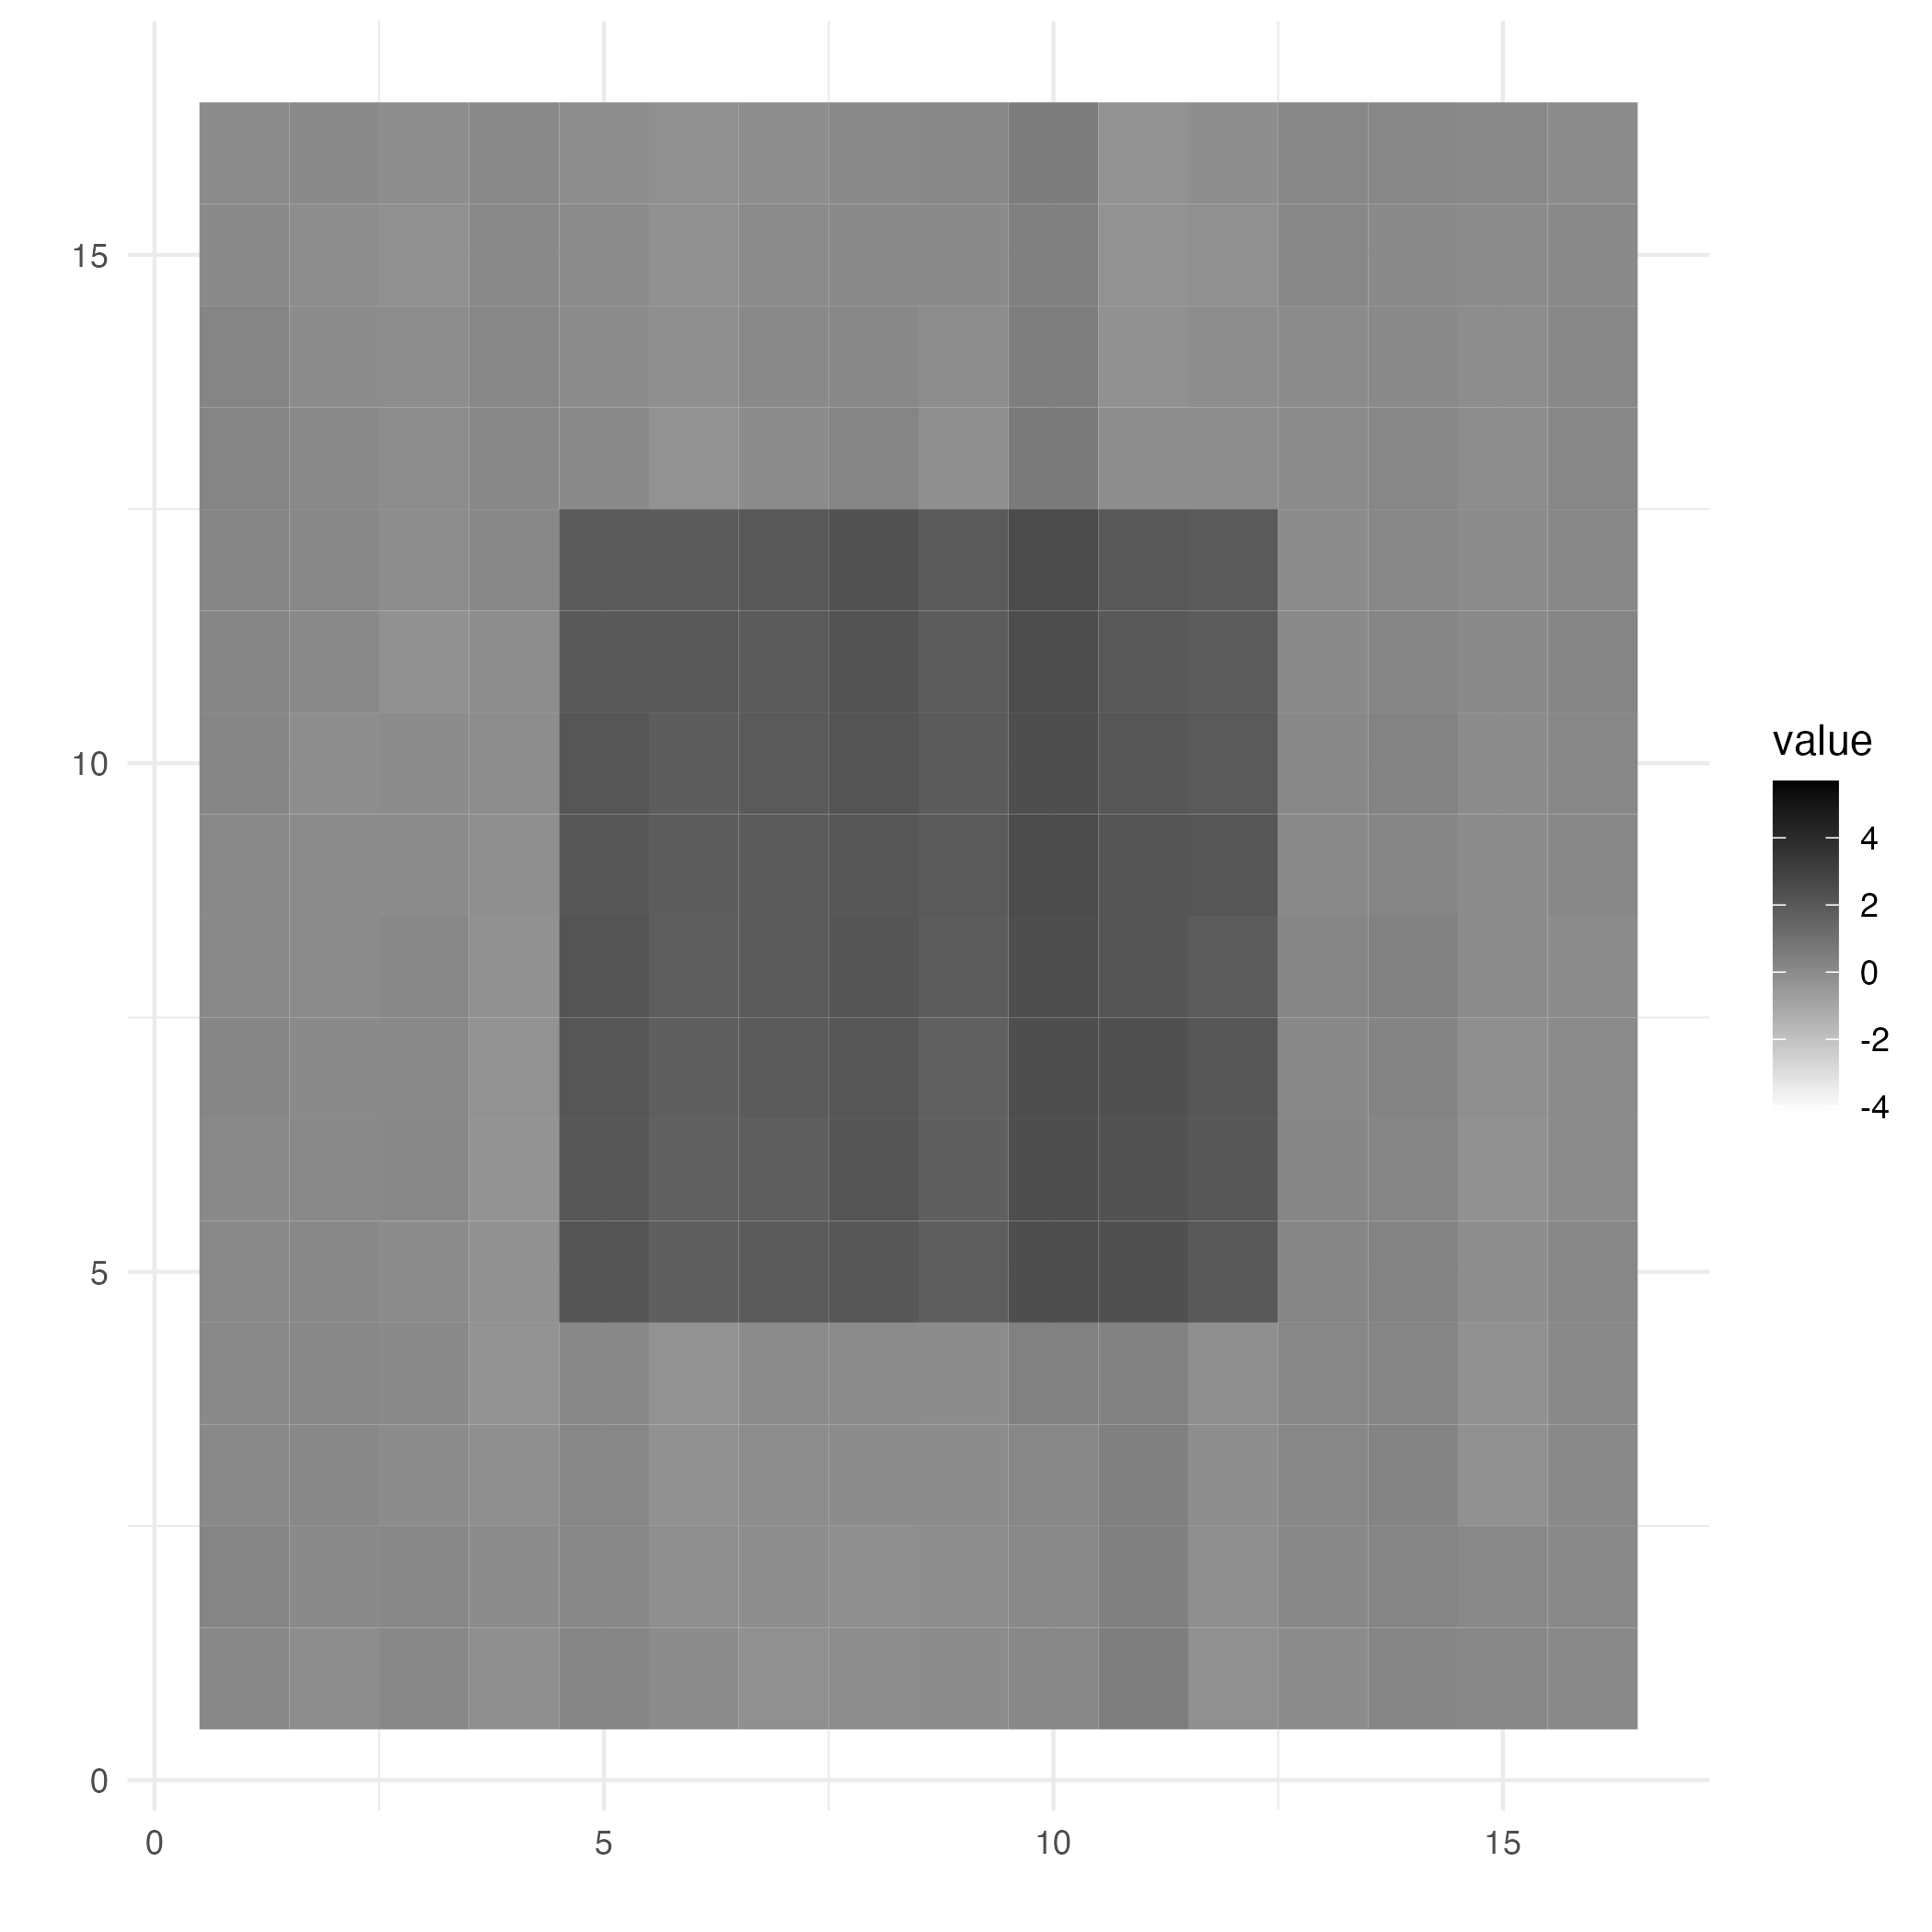
\includegraphics[width=\textwidth]{/Users/siyangren/Documents/ra-cida/ESFGSP_Paper/Figures/image_ex2.png}
    \end{minipage}
\end{figure}

\section*{spVBM}

The spVBM model is:
\[
    \begin{aligned}
         & y_s^i=\sum_{k=1}^K x_{s, k}^i \beta_{s, k}^{S V C}+\mathbf{Z}^{\mathbf{i}} \mathbf{b}^{\mathbf{i}}+\varepsilon_s^i                                                                                                                      \\
         & \beta_{s, k}^{S V C}=\beta_k+[\mathbf{E} \Gamma]_{s, k}                                                                                                                                                                                 \\
         & \mathbf{b}^{\mathbf{i}} \sim \mathcal{N}(\mathbf{0}, G), \quad \varepsilon_i \sim \mathcal{N}\left(0, \sigma^2\right), \quad \Gamma_{, k} \sim \mathcal{N}\left(\mathbf{0}, \sigma_k^2 \boldsymbol{\Lambda}\left(\alpha_k\right)\right)
    \end{aligned}
\]
\(y_s^i\) denote the spatial outcome for subject \(i\) voxel \(s\). \(\mathbf{Z}\) denote non-spatial subject-level covariates for non-spatial random effects.

In our simulated data, this could be simplified to \(y_s^i = x_s^i \beta_s^{SVC} + (?) \). My question is, which term captures the exponential correlation structure in the model? \(G\) or \(\Gamma\)?

\begin{figure}[ht]
    \centering
    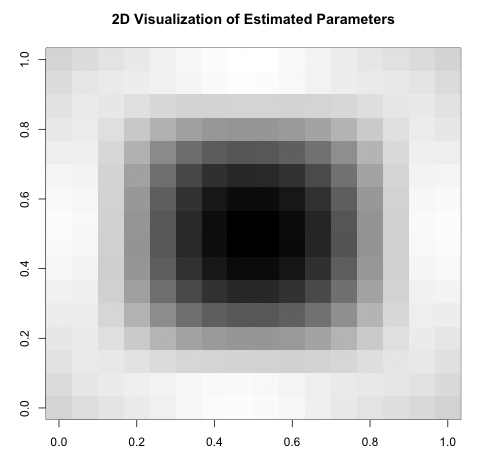
\includegraphics[width=0.5\textwidth]{/Users/siyangren/Documents/ra-cida/ESFGSP_Paper/Figures/spvbm_coefs_april_3.png}
    \caption{Estimated coefficients}
    \label{fig:my_label}
\end{figure}


\end{document}
